\documentclass[12pt]{scrartcl}

\usepackage{fullpage}
\usepackage{graphicx}
\spac

\title{Honors Thesis}
\author{Gina Chun}


\begin{document}

\maketitle

\newpage

\begin{abstract}
  Abstract...
\end{abstract}

\newpage

\tableofcontents

\newpage

\section{Introduction}\label{Introduction}



\subsection{why carbon is important}\label{Test}

% In this section to say blah

Carbon is one of the most important and widely investigated
elements. Carbon is all around us in a variety of forms and is an area
of study which has huge significance across many scientific fields and
applications. Carbon is in living organisms and is essential for
living organisms, thus the study of carbon would further develop the
complex workings of the environment, ecosystems and the carbon
cycle. It would also help the understanding of fossil fuels, aid the
challenges of energy-related issues, and work towards solutions for
climate change. Carbon materials are also intertwined in modern
economic industries such as in steel, clothing, pigment, plastic and
synthetic materials, and in electrodes and other similar electricity
conducting machinery. Studying carbon allows for further advancement
in these important industries which would lead to better and more
easily accessible devices, tools, and products for general society.

Now referencing the introduction \ref{Test}

\subsection{why use machine learning}
As carbon is an important element, its versatility makes it a very
complex subject of study. Carbon manifests in various physical forms,
called allotropes, each with very different properties. Because of
this, studying carbon can be difficult with conventional
methods. Using Gaussian Approximation Potentials (GAP), machine
learning can be much more cost and time efficient than traditional
scientific methods of experimentation. Machine learning also opens up
a new space of empirical methods for experiments that scientists
cannot physically replicate with traditional techniques. For example,
machine learning can be used for experiments in very small spatial
scales or for large scale simulations all while maintaining high
performance accuracy.

Here is an example of a citation: \cite{gap20}, \cite{DGL}

\newpage

\section{Background}

\subsection{Chemistry}
\begin{itemize}
    \item[!] Machine Learning Meets Quantum Physics textbook
\end{itemize}

% Introduction to material modeling
Using machine learning to study any kind of material, not just carbon, 
is just one method under a wider category of techniques called material modeling. 
Material modeling in chemistry is the method of using computer simulations to predict 
physical and chemical properties of a material in replace of real-world experiments. 
This process of predicting the properties of a given material is called a \emph{forward 
problem}. Through existing tools such as statistical mechanics and the Schrödinger 
equation, which will be talked about later, an exact unique solution exists for the 
forward problem of predicting material properties and is the reason why many opt to 
use this procedure. Material modeling also uses this approach because the inverse 
problem, constructing a material through a set of pre-determined properties, 
is much more difficult and costly to do.

\subsubsection{Geometry and Structure}
% Structure property relation for molecules
``Structure determines properties'' is a very important and central concept in chemistry. 
This structure-property relationship explains that since all materials are made of atoms, identifying 
and describing a material comes down to simply understanding its atomic structure. For studying 
structures, there is never a need to look at the entire material as well. That would be too many 
atoms to study at once and atoms of most solid materials, like crystalline carbon, are arranged in 
an organized repetitive pattern so it is sufficient enough to look at just a patch of that pattern. 
Studying the properties of a microscopic structure, in general, translates well to its macroscopic 
structure which allows it to pair well with the material modeling approach.

% molecular \& material properties: Electronic properties (for hard degrees of freedom, crystalline)
% Born–Oppenheimer approximation, ground state, atomization energy
An atom can be described as having a heavy nucleus surrounded by a cloud of light 
electrons and since the mass of an atom is concentrated on its nucleus, the atom's 
position is associated with the position of the nucleus. Thus moving atoms can be described
as moving nuclei being followed by their clouds of electrons. The Born–Oppenheimer 
approximation is the mathematical formulation of this concept and is the foundation 
of material modeling. Molecular and material properties can be roughly divided into 
two categories: electronic and thermodynamic properties.Electronic properties are 
essentially the properties of that electron cloud that is following the nucleus and 
is best described through quantum mechanics, which will be covered in more detail later. 
To give a general overview, the electronic cloud can be in certain states such as its 
lowest-energy state called the \emph{ground state}. Some ground state properties include the
atomization energy, which is the energy released when a molecule is formed, and the 
dipole moment and polarizability, which describes the shape and responsiveness of the
cloud. Since thermodynamic properties can be more easily derived through knowing the electronic 
properties first, this paper and its method will be predicting ground-state electronic properties 
so that is what the background will be focused on. 


\subsubsection{Quantum Mechanics}
% object being in multiple states
% Schrödinger equation, DFT, PES
% computational cost with solving the equation
Quantum mechanics is the set of laws that describe objects on an atomic level. One of the core
principles is that an object can be in multiple states. An object like an electron can be in any 
combination of these two states. Mathematically, this can be expressed as a linear combination of 
two basis vectors that act as the two position states. The state of this object can be expressed 
as a \emph{wave function}, which generalizes the two position vectors to the infinite number of 
positions in the three-dimensional space. This fundamental idea is why electrons are commonly 
referred to as clouds.

The laws of quantum mechanics also states that each observable, quantifiable, physical property that 
an atomic object has is associated with a linear operator. The actual value of the quantity is given 
by the eignevalues of the operator. One of the most important operators is the energy operator, called 
the Hamiltonian, and its associated eigenvalue equation is called a Schrödinger equation. The energy of 
a particular eigenstate as a function of the nuclear positions is called a \emph{potential energy surface}
and it completely determines the dynamics of the motion of the atoms. The solution to this equation 
allows many electronic properties of both ground and excited states to be determined. The Schrödinger 
equation can be mathematically solved for singular atoms but it gets more difficult for more complex molecules. 
There are methods such as the density functional theory and the Hartree-Fock that try to 
solve this issue by manipulating the Hamiltonian or the vector space itself, but their computational 
costs make these methods practically inefficient. Once the Schrödinger equation is solved, evaluating 
properties such as atomization energy or dipole moment can be done through the eigenvalues and eigenstates.


\newpage


\subsection{Machine Learning}
\begin{itemize}
    \item[!] https://distill.pub/2021/gnn-intro/
\end{itemize}
\subsubsection{Graph Represented Data}
\begin{itemize}
    \item graph representation (molecules as graphs)
    \item types of problems that use graph structured data 
    \item integrating graphs in neural networks (matrices, adjacency lists)
\end{itemize}
\subsubsection{Graph Neural Networks}    
\begin{itemize}
    \item formal definition of graph neural networks
    \item Graphic convolution
    \item pooling
    \item message passing
    \begin{itemize}
        \item https://dl.acm.org/doi/10.5555/3305381.3305512
        \item Machine Learning Meets Quantum Physics textbook Ch 10
    \end{itemize}
\end{itemize}

%\begin{figure}
  %\centering
  %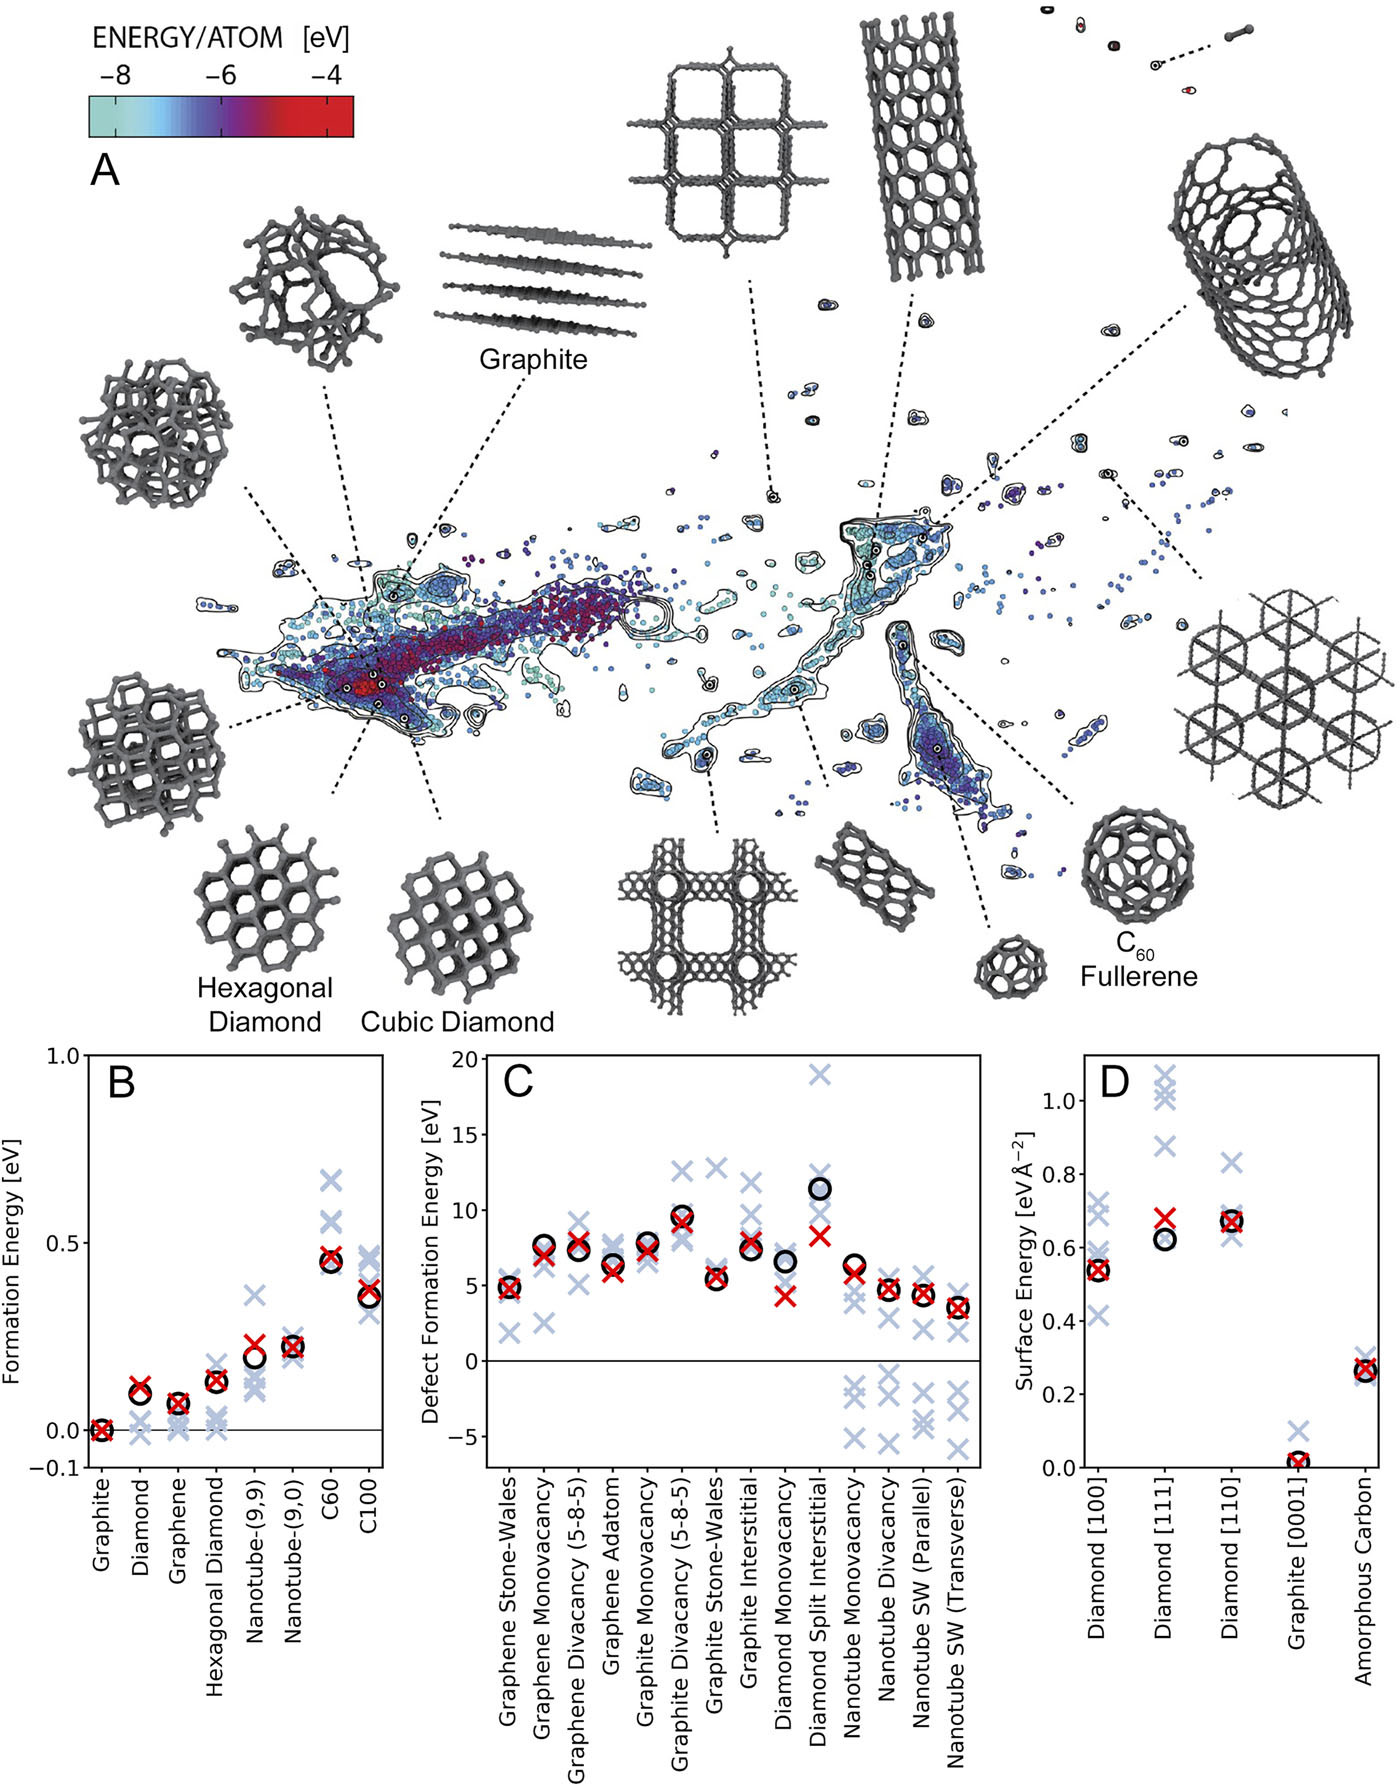
\includegraphics[scale=2]{carbon}
  
  %\caption{Nice caption}\label{fig:my_figure}
%\end{figure}


%In figure \ref{fig:my_figure}


\newpage 

\section{Method}
\subsubsection{Carbon GAP 20 dataset (describe, why)}  
\subsubsection{graph model (describe, why)}  
Not permutation invariance yet?
\newline The model itself is semi permutation invariant but the local environments must be permutation invariant for the model to be COMPLETELY permutation invariant
\newline Also columb matrix creating rotation and translation invariance in paper
\newline What if everyone becomes the neighbors: How the local level is more important
 


\newpage

\section{Experimental Evaluation}
\subsubsection{other experiments}  
\begin{itemize}
    \item papers citing GAP 20
    \item Data-efficient iterative training of Gaussian approximation potentials: Application to surface structure determination of rutile IrO2 and RuO2 (https://aip.scitation.org/doi/abs/10.1063/5.0071249)
    \item A comprehensive assessment of empirical potentials for carbon materials (https://aip.scitation.org/doi/abs/10.1063/5.0052870)
    \item Transferability of machine learning potentials: Protonated water neural network potential applied to the protonated water hexamer (https://aip.scitation.org/doi/full/10.1063/5.0035438)
    \item Machine learning interatomic potential developed for molecular simulations on thermal properties of Beta-Ga2O3 (https://aip.scitation.org/doi/abs/10.1063/5.0027643)
\end{itemize}
\newpage

\section{Conclusion}

\newpage

\bibliographystyle{plain}
\bibliography{ref}


\end{document}
